   \node (plotCenter) at (-2,-2.4){};
   \node [scale=1,anchor=south] at (plotCenter.center){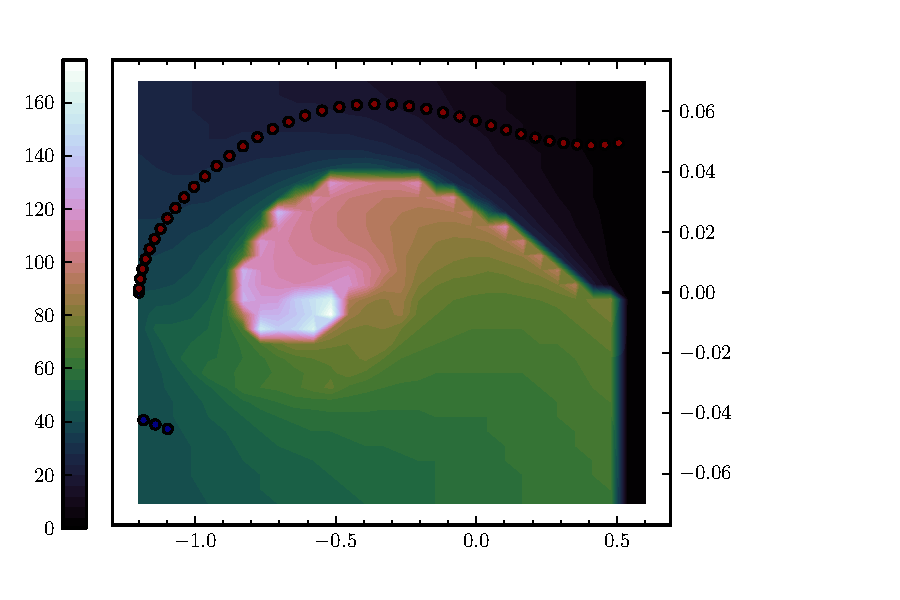
\includegraphics{Figures/Mountain_car_Expert_traj_length.pdf}};
   \node[red] (plotMark) at ($(plotCenter.center) + (0.59,8)$) {\huge \bf x};
   \draw [thick,red,dotted](plotMark.center) -- ++(0,-6.6);
   \draw [thick,red,dotted](plotMark.center) -- ++(3,0);
   
   \node (mcSW) at (4,-1){};
  %Mountain car
  \draw  [ultra thick] (mcSW)++(0,6) sin ++(5,-5) cos ++(5,5) sin ++(5,5);
  \fill[green!50] (mcSW.center)-- ++(0,6) sin ++(5,-5) cos ++(5,5) sin ++(5,5) -- ++(0,-11) --cycle;
  %\draw (0,-1) grid (20,10);
 \node (tuture)[scale=1,rotate=55,anchor=south]at ($(mcSW)+(10.38,6.5)$) {\usebox\tuture};
 \node [scale=1,rotate=55,anchor=south,scale=1.4](speedArrow)at ($(mcSW)+(9.8,6.9)$) {\speedarrow{48}};
 \draw [very thin] (mcSW.center) -- ++(15,0);
 \foreach \x in {0,1,...,15}{
   \draw (mcSW.center) ++(\x,0) -- ++(0,.05);
 }
 \foreach \x in {-1,-0.5,0.0,0.5}{
   \draw (mcSW.center) ++($10*(\x+1,0)$) -- ++(0,.15);
   \node at ($(mcSW.center) +10*(\x+1,-.03)$) {$\x$};
 }


 \draw [thick,red,dotted]($(tuture.center)+(0,-0.15)$) -- ++(0,-6.5);
 \draw [red,<->]($(mcSW.center)+(10,-0.6)$) -- ++(0,-1) -- ($(plotMark.center)+(0,-8.2)$) -- ++(0,1);
 \draw [thick,red,decorate,decoration=brace,rotate=55] ($(speedArrow)+(-.7,0.2)$) -- ++(1.4,0);
 
 \draw [red,<->]($(speedArrow.center)+(-.7,0.2)$)  -- ($(plotMark.center)+(3.5,0)$);

